\documentclass[
11pt, % Set the default font size, options include: 8pt, 9pt, 10pt, 11pt, 12pt, 14pt, 17pt, 20pt
%t, % Uncomment to vertically align all slide content to the top of the slide, rather than the default centered
%aspectratio=169, % Uncomment to set the aspect ratio to a 16:9 ratio which matches the aspect ratio of 1080p and 4K screens and projectors
]{beamer}

\graphicspath{{Images/}{./}} % Specifies where to look for included images (trailing slash required)

\usepackage{todonotes}
\usepackage{graphicx}
\usepackage{xcolor}
\usepackage{subfig}
%%\usepackage[noend]{algpseudocode}

%
%\usepackage{algorithm}
%\usepackage{algorithmic}
\usepackage{algorithm}
\usepackage{algpseudocode}
\usepackage{blkarray}
\usepackage{amsmath}
\usepackage{xspace}
\usepackage{float}


\usepackage{tikz}
\usetikzlibrary{matrix, decorations, patterns, positioning, shapes, calc, intersections, arrows, fit}

\usetikzlibrary{patterns}
\usetikzlibrary{fit,calc,positioning,decorations.pathreplacing,matrix,3d, hobby}

\usepackage{booktabs} % Allows the use of \toprule, \midrule and \bottomrule for better rules in tables
\usepackage{bm}
\usepackage{multirow}
\usepackage{ragged2e}


\newcommand{\brown}[1]{{\color{brown} #1 }}

%% Colors from https://latexcolor.com/
\definecolor{pastelviolet}{rgb}{0.8, 0.6, 0.79}
\definecolor{babyblueeyes}{rgb}{0.63, 0.79, 0.95}
\definecolor{pastelyellow}{rgb}{0.99, 0.99, 0.59}
\definecolor{pastelgreen}{rgb}{0.47, 0.87, 0.47}
\definecolor{pastelred}{rgb}{1.0, 0.41, 0.38}
\colorlet{patternblue}{blue!60}



%%\newcommand{\tensorcolor}{patternblue}
\newcommand{\tensorcolor}{cyan}


\colorlet{darkred}{red!80!black}
\colorlet{darkblue}{blue!80!black}
\newcommand<>{\darkred}[1]{{\color{darkred}{#1}}}
\newcommand<>{\darkblue}[1]{{\color#2{blue!50!black!100}{#1}}}

\newcommand{\A}{\mathbf{A}}
\newcommand{\B}{\mathbf{B}}
\newcommand{\CC}{\mathbf{C}}
%\newcommand{\Real}{\mathbb{R}}
%\newcommand{\vc}[1]{\bm{#1}}

\usetheme{Madrid}

%\newcommand{\Tra}{{\sf T}} 


%\newcommand{\Ms}[2]{\mathbf{#1}^{(#2)}} 
%\newcommand{\M}[1]{\mathbf{#1}} 
%\newcommand{\Mb}[2]{\mathbf{#1}_{#2}} 
%\newcommand{\Mbs}[3]{\mathbf{#1}_{#2}^{(#3)}} 

%\usepackage{enumitem}

\input{../tensor_header}

\newcommand{\X}{\T{X}}
\newcommand{\Y}{\T{Y}}

\newcommand{\starontop}[1]{{#1}^*}

\hypersetup{linkcolor=blue}

%----------------------------------------------------------------------------------------
%	PRESENTATION INFORMATION
%----------------------------------------------------------------------------------------

\title[Multi-TTM]{Multiple Tensor Times Matrix computation} % The short title in the optional parameter appears at the bottom of every slide, the full title in the main parameter is only on the title page

%\subtitle{Optional Subtitle} % Presentation subtitle, remove this command if a subtitle isn't required

\author[Suraj Kumar]{Suraj Kumar} % Presenter name(s), the optional parameter can contain a shortened version to appear on the bottom of every slide, while the main parameter will appear on the title slide

\institute[Inria \& ENS Lyon]{Inria \& ENS Lyon \\ \smallskip Email:\textit{suraj.kumar@inria.fr}} % Your institution, the optional parameter can be used for the institution shorthand and will appear on the bottom of every slide after author names, while the required parameter is used on the title slide and can include your email address or additional information on separate lines

\date[CR12]{CR12: October 2023\\ \smallskip\small https://surakuma.github.io/courses/daamtc.html} % Presentation date or conference/meeting name, the optional parameter can contain a shortened version to appear on the bottom of every slide, while the required parameter value is output to the title slide

%----------------------------------------------------------------------------------------

\begin{document}
	
	%----------------------------------------------------------------------------------------
	%	TITLE SLIDE
	%----------------------------------------------------------------------------------------
	
	\begin{frame}
		\titlepage % Output the title slide, automatically created using the text entered in the PRESENTATION INFORMATION block above
	\end{frame}

\begin{frame}{Tucker decomposition of $\T{A} \in \mathbb{R}^{n_1\times n_2\times\cdots\times n_d}$}
	
	\small
	It represents a tensor with $d$ matrices (usually orthonormal) and a small core tensor.
	\vspace*{-0.25cm}\begin{center}
		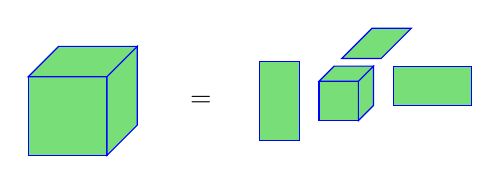
\begin{tikzpicture}[scale=0.25, every node/.style={transform shape}]
		\pgfmathsetmacro{\cubex}{4}
		\pgfmathsetmacro{\cubey}{4}
		\pgfmathsetmacro{\cubez}{4}
		\draw[blue,fill=pastelgreen] (-12,1,\cubez-2) -- ++(-\cubex,0,0) -- ++(0,-\cubey,0) -- ++(\cubex,0,0) -- cycle;
		\draw[blue,fill=pastelgreen] (-12,1,\cubez-2) -- ++(0,0,-\cubez) -- ++(0,-\cubey,0) -- ++(0,0,\cubez) -- cycle;
		\draw[blue,fill=pastelgreen] (-12,1,\cubez-2) -- ++(-\cubex,0,0) -- ++(0,0,-\cubez) -- ++(\cubex,0,0) -- cycle;
		\node[draw=none, text=black, scale=4] at (-8,-1,0) {$=$};
		
		\pgfmathsetmacro{\cubex}{2}
		\pgfmathsetmacro{\cubey}{2}
		\pgfmathsetmacro{\cubez}{2}
		\draw[blue,fill=pastelgreen] (0,0,0) -- ++(-\cubex,0,0) -- ++(0,-\cubey,0) -- ++(\cubex,0,0) -- cycle;
		\draw[blue,fill=pastelgreen] (0,0,0) -- ++(0,0,-\cubez) -- ++(0,-\cubey,0) -- ++(0,0,\cubez) -- cycle;
		\draw[blue,fill=pastelgreen] (0,0,0) -- ++(-\cubex,0,0) -- ++(0,0,-\cubez) -- ++(\cubex,0,0) -- cycle;
		
		\draw[blue,fill=pastelgreen] (-\cubex-1,1,0) -- ++(-\cubex,0,0) -- ++(0,-\cubey-2,0) -- ++(\cubex,0,0) -- cycle;
		\draw[blue,fill=pastelgreen] (\cubex+2+1,0,-\cubey) -- ++(-\cubex-2,0,0) -- ++(0,-\cubey,0) -- ++(\cubex+2,0,0) -- cycle;
		
		\draw[blue,fill=pastelgreen] (0,0,-\cubez-1) -- ++(-\cubex,0,0) -- ++(0,0,-\cubez-2) -- ++(\cubex,0,0) -- cycle;
		\end{tikzpicture}
	\end{center}
	\vspace*{-0.15cm}\centering{\footnotesize Tucker decomposition of a $3$-dimensional tensor.}
	\vfill
	{\footnotesize\vspace*{-0.1cm}$$\T{A} = \T{G} \times_1 U_1 \cdots \times_d U_d$$
		$$\T{A}(i_1,\cdots,i_d) = \sum_{\alpha_1=1}^{r_1}\cdots\sum_{\alpha_d=1}^{r_d} \T{G}(\alpha_1,\cdots,\alpha_d)U_1(i_1,\alpha_1)\cdots U_d(i_d, \alpha_d)$$}
	\vfill
	\justifying
	It can be concisely expressed as $\T{A} = \llbracket \T{G}; U_1, \cdots, U_d\rrbracket $.
	\vfill
	Here $r_j$ for $1\le j\le d$ denote a set of ranks. Matrices $U_j \in \mathbb{R}^{n_j\times r_j}$ for $1\le j \le d$ are usually orthonormal and known as factor matrices. The tensor $\T{G}\in \mathbb{R}^{r_1\times r_2\times\cdots\times r_d}$ is called the core tensor. 	
\end{frame}

\begin{frame}{\large High Order SVD (HOSVD) for computing a Tucker decomposition}
	\small
	\begin{algorithm}[H]{
			\caption{HOSVD method to compute a Tucker decomposition}
			\begin{algorithmic}[1]
				\Require input tensor $\T{A}\in \mathbb{R}^{n_1\times \cdots \times n_d}$, desired rank $(r_1,\cdots, r_d)$
				\Ensure  $\T{A} = \T{G} \times_1 U_1 \times_2 U_2  \cdots \times_d U_d$
				\For{$k=1 \text{ to } d$}
				\State $U_k \gets r_k$ leading left singular vectors of $A_{(k)}$
				\EndFor
				\State $\T{G} = \T{A} \times_1 U_1^\Tra \times_2 U_2^\Tra  \cdots \times_d U_d^\Tra$
			\end{algorithmic}
	}\end{algorithm}
	
	
	\vfill
	\begin{itemize}
		\item When $r_i < rank(A_{(i)})$ for one or more $i$, the decomposition is called the truncated-HOSVD (T-HOSVD)
		\vfill
		\item The collective operation $\T{A} \times_1 U_1^\Tra \times_2 U_2^\Tra  \cdots \times_d U_d^\Tra$ is known as Multiple Tensor-Times-Matrix (Multi-TTM) computation
	\end{itemize}
\end{frame}
\begin{frame}{\large Sequentially T-HOSVD (ST-HOSVD) for Tucker decomposition}
	\small
	\begin{itemize}
		\item This method is more work efficient than T-HOSVD
		\vfill
		\item In each step, it reduces the size of one dimension of the tensor
	\end{itemize}
	
	%	\small
	\vspace{-0.25cm}\begin{algorithm}[H]{
			\caption{ST-HOSVD method to compute a Tucker decomposition}
			\begin{algorithmic}[1]
				\Require input tensor $\T{A}\in \mathbb{R}^{n_1\times \cdots \times n_d}$, desired rank $(r_1,\cdots, r_d)$
				\Ensure  $\llbracket \T{G}; U_1, \cdots, U_d\rrbracket $ : a $(r_1, \cdots, r_d)$-rank Tucker decomposition of $\T{A}$
				\State $\T{B} \gets \T{A}$
				\For{$k=1 \text{ to } d$}
%				\State $S\gets B_{(k)}B_{(k)}^T$
				\State $U_k \gets r_k$ leading singular vectors of $B_{(k)}$
				\State $\T{B} \gets \T{B} \times_k U_k$
				\EndFor
				\State $\T{G} = \T{B}$
			\end{algorithmic}
	}\end{algorithm}
%\vspace{-0.215cm}
We can note that ST-HOSVD also performs Multi-TTM computation by doing a sequence of TTM operations, i.e, $\T{G} =((\T{A} \times_1 U_1)\times_2 U_2) \cdots \times_d U_d $.
\end{frame}

\begin{frame}{\large Bottlenecks for algorithms to compute Tucker decompositions}
	\vfill
	\begin{itemize}
		\item Multi-TTM becomes the overwhelming bottleneck computation when
		\vfill
		\begin{itemize}
			\item Matrix SVD costs are reduced using randomization via sketching or
			\vfill
			\item $U_k$ are computed with eigen value decompositions of $B_{(k)}B_{(k)}^T$
		\end{itemize}   
	\end{itemize}
\vfill
\end{frame}
%\begin{frame}{}
%	content...
%\end{frame}



\begin{frame}{Multi-TTM computation}
	\small
	Let $\Y\in \mathbb{R}^{r_1\times\cdots\times r_d}$ be the output tensor, $\X\in \mathbb{R}^{n_1\times\cdots\times n_d}$ be the input tensor, and $\Mn{A}{k} \in \mathbb{R}^{n_k\times r_k}$ be the matrix of the $k$th mode. Then the Multi-TTM computation can be represented as 
	\vspace*{-0.25cm}$$\Y = \X \times_1 {\Mn{A}{1}}^\Tra \cdots \times_d {\Mn{A}{d}}^\Tra$$
	$$\text{ or }\X = \Y \times_1 {\Mn{A}{1}} \cdots \times_d {\Mn{A}{d}}\text.$$
	
	We will focus only on the first representation in this course. Our results and analysis extend straightforwardly to the latter case.
	
	\vfill
	\emph{Two approaches to perform this computation}:
	\begin{itemize}
		\item TTM-in-Sequence approach -- performed by a sequence of TTM operations
		\vspace*{-0.15cm}$$\Y = ((\X \times_1 {\Mn{A}{1}}^\Tra)\times_2 {\Mn{A}{2}}^\Tra) \cdots \times_d {\Mn{A}{d}}^\Tra$$
	\vfill
		\item All-at-once approach
		\vspace*{-0.15cm}$$\Y(r_1^\prime,\ldots,r_d^\prime) = \sum_{\{n_k^\prime \in [n_k]\}_{k \in [d]}} \X(n_1^\prime,\ldots,n_d^\prime) \prod_{j \in [d]} \Mn{A}{j}(n_j^\prime,r_j^\prime)$$
	\end{itemize}
	\vfill
	$[d]$ denotes $\{1,2,\cdots, d\}$. We represent $n_1n_2\cdots n_d$ and $r_1r_2\cdots r_d$  by $n$ and $r$ respectively. We mainly focus on all-at-once approach.
%	 This approach reduces communication.
\end{frame}

\begin{frame}{Final assignment -- deadline Oct 24}
	\vfill
\brown{Question:} Let $\Y\in \mathbb{R}^{r\times r \times r \times r}$, $\X\in \mathbb{R}^{n \times n \times n \times n}$ and $A \in \mathbb{R}^{n\times r}$. What are the different approaches to perform the following Multi-TTM computation: 
$$\Y = \X \times_1 A^\Tra \times_2 A^\Tra \times_3 A^\Tra  \times_4 A^\Tra $$
Compute the exact number of arithmetic operation for each approach.
\vfill
\end{frame}



\section{Parallel Multi-TTM computation}
	\begin{frame}{Table of Contents}		
		\tableofcontents[currentsection,hideallsubsections] % Output the table of contents (all sections on one slide)
		\begin{block}{Settings to compute parallel communication lower bound}
			\small
			\begin{itemize}
				\item Without loss of generality, we assume that $n_1r_1\le n_2r_2\le \cdots \le n_dr_d$
				\vfill
				\item The input tensor is larger than the output tensor, i.e., $n\ge r$
				\vfill
				\item The algorithm load balances the computation -- each processor performs $1/P$th number of loop iterations
				\vfill
				\item One copy of data is in the system
				\begin{itemize}
					\item There exists a processor whose input data at the start plus output data
					at the end must be at most $\frac{n + r + \sum_{i=1}^{d}n_ir_i }{P}$ words – will analyze amount of data
					transfers for this processor
				\end{itemize}
			\end{itemize}
		\end{block}		
	\end{frame}

\subsection{$3$-dimensional Multi-TTM}
	\begin{frame}{Table of Contents}		
	\tableofcontents[currentsection,currentsubsection] % Output the table of contents (all sections on one slide)		
\end{frame}

\begin{frame}{Optimization problems (Ballard et. al., 2023)}
	\footnotesize
\vspace*{-0.25cm}\begin{lemma}
	Consider the following optimization problem:
	\vspace*{-0.15cm}$$\min_{x,y,z} x+y+z \text{ such that }$$ 
	\vspace*{-0.15cm}$$\frac{nr}{P} \le xyz, \quad
	0 \le \phantom{y}x\phantom{z} \le n_1r_1,\quad
	0 \le \phantom{x}y\phantom{z} \le n_2r_2, \quad 
	0 \le \phantom{x}z\phantom{y} \le n_3r_3,$$
%	\begin{align*}
%	\frac{nr}{P} &\le xyz  \\ 
%	,
%	\end{align*}
	where $n_1r_1 \le n_2r_2 \le n_3r_3$, and $n_1,n_2,n_3,r_1,r_2,r_3,P \ge 1$.
	The optimal solution $(\starontop{x},\starontop{y},\starontop{z})$ depends on the relative values of the constraints, yielding three cases:
	\begin{enumerate}
		\item if $P < \frac{n_3r_3}{n_2r_2}$, then $\starontop{x}=n_1r_1$, $\starontop{y}=n_2r_2$, $\starontop{z}=\frac{n_3r_3}{P}$;
		\item if $\frac{n_3r_3}{n_2r_2}\le P < \frac{n_2n_3r_2r_3}{n_1^2r_1^2}$, then $\starontop{x}=n_1r_1$, $\starontop{y}=\starontop{z}= \big(\frac{n_2n_3r_2r_3}{P}\big)^{\frac{1}{2}}$;
		\item if $\frac{n_2n_3r_2r_3}{n_1^2r_1^2} \le P$, then $\starontop{x}=\starontop{y}=\starontop{z}= \big(\frac{nr}{P}\big)^{\frac{1}{3}}$;
	\end{enumerate}
	which can be visualized as follows.
	\vspace*{-0.35cm}\begin{center}
		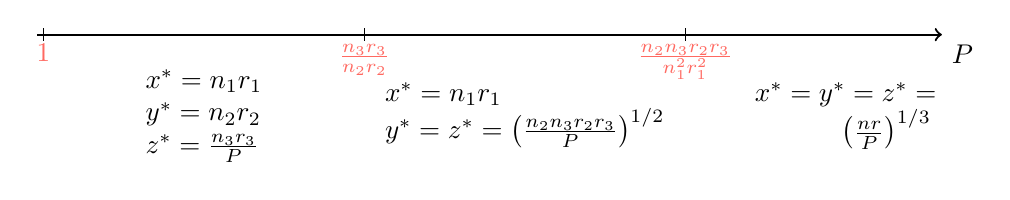
\begin{tikzpicture}[scale=0.815, every node/.style={transform shape}]
		\draw [->, thick] (-0.1,0) -- (14,0) node [below right, scale=1.2] {$P$};
		\draw (0, 0.1) -- node [below, pastelred, scale=1.2]{$1$}(0,-0.1);
		\draw (5, 0.1) -- node [below, pastelred, scale=1.2]{$\frac{n_3r_3}{n_2r_2}$}(5,-0.1);
		\draw (10, 0.1) -- node [below, pastelred, scale=1.2] {$\frac{n_2n_3r_2r_3}{n_1^2r_1^2}$}(10,-0.1);
		
		\node[align=left,below,scale=1.2] at (2.5, -0.4) {$\starontop{x}=n_1r_1$\\ $\starontop{y}=n_2r_2$\\ $\starontop{z}=\frac{n_3r_3}{P}$};
		\node[align=left,below,scale=1.2] at (7.5, -0.6) {$\starontop{x}=n_1r_1$\\$\starontop{y}=\starontop{z}= \big(\frac{n_2n_3r_2r_3}{P}\big)^{1/2}$};
		\node[align=center,below,scale=1.2] at (12.5, -0.6) {$\starontop{x}=\starontop{y}=\starontop{z}=$\\ $\qquad\quad \big(\frac{nr}{P}\big)^{1/3}$};	
		\end{tikzpicture}
	\end{center} 
\end{lemma}
\end{frame}
\begin{frame}{Optimization problems (Ballard et. al., 2023)}
	\footnotesize
	\begin{lemma}
		Consider the following optimization problem:
		\vspace*{-0.15cm}$$\min_{u,v} u+v \text{ such that }$$
		\vspace*{-0.15cm}$$\frac{nr}{P} \le uv, \quad 
		0 \le \;u\; \le r, \quad 
		0 \le \;v\; \le n,$$
		where $n\geq r$, and $n,r,P \ge 1$.
		The optimal solution $(\starontop{u},\starontop{v})$ depends on the relative values of the constraints, yielding two cases:
		\begin{enumerate}
			\item if $P < \frac{n}{r}$, then $\starontop{u}= r$, $\starontop{v} = \frac{n}{P}$;
			\item if $ \frac{n}{r} \le P$, then $\starontop{u}=\starontop{v}= \big(\frac{nr}{P}\big)^{\frac{1}{2}}$;
		\end{enumerate}
		which can be visualized as follows.
		\vspace*{-0.35cm}\begin{center}
			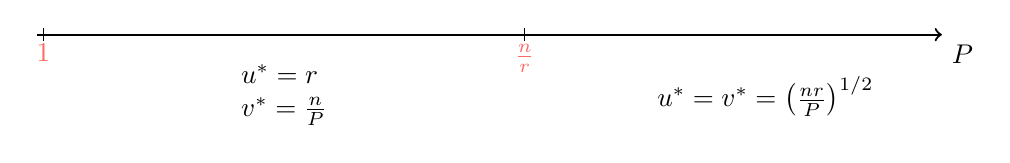
\begin{tikzpicture}[scale=0.815, every node/.style={transform shape}]
			\draw [->, thick] (-0.1,0) -- (14,0) node [below right, scale=1.2] {$P$};
			\draw (0, 0.1) -- node [below, pastelred, scale=1.2]{$1$}(0,-0.1);
			\draw (7.5, 0.1) -- node [below, pastelred, scale=1.2]{$\frac{n}{r}$}(7.5,-0.1);
			
			\node[align=left,below,scale=1.2] at (3.75, -0.325) {$\starontop{u}= r$\\ $\starontop{v} = \frac{n}{P}$};
			\node[align=left,below,scale=1.2] at (11.25, -0.5) {$\starontop{u}=\starontop{v}= \big(\frac{nr}{P}\big)^{1/2}$};
			\end{tikzpicture}
		\end{center} 
	\end{lemma}
	Both lemma can be proved using the KKT conditions.
\end{frame}

\subsection{$d$-dimensional Multi-TTM}
\begin{frame}{Table of Contents}		
	\tableofcontents[currentsection,currentsubsection] % Output the table of contents (all sections on one slide)		
\end{frame}

\end{document} 